\documentclass{beamer}
\usetheme{metropolis}
%%%
\usepackage{polyglossia}
\setmainlanguage{spanish}
\setotherlanguages{english}
%%%
\usepackage{url}
\usepackage{lscape}
\usepackage[squaren]{SIunits}
\usepackage{spverbatim}
%%%
\usepackage{csquotes}
\usepackage[style=authoryear-comp, backend=bibtex]{biblatex} 
% \bibliographystyle{plainnatR} 
% backend=biber  % for biber
% apalike harvard chicago unsrtnat elsart-num-names
% \bibliography{referencias}
\addbibresource{referencias.bib}
%%%
% R/knitr
\usepackage{tikz}
\usepackage{rotating}
\usepackage{subfig}
\usepackage{inconsolata}
\usepackage{dcolumn}   % requerido por stargazer y texreg
\usepackage{booktabs}  % requerido por xtable y texreg
%%%
\usepackage{syntonly}
%\syntaxonly %verifica sintaxis sin generar documento
%%%

%%%%%%%%%%%%%%%%%% hipervinculos activos %%%%%%%%%%%%%%%%%%%%%%%

% \ifx\pdfoutput\undefined % We're not running pdftex
% \RequirePackage[bookmarks,hyperindex,plainpages=false]{hyperref}
% %colorlinks,
% \else
% \RequirePackage[bookmarks,hyperindex,plainpages=false]{hyperref}
% \def\pdfBorderAttrs{/Border [0 0 0] } % No border arround Links
% \hypersetup{pdfauthor={Ulises M. Alvarez}}
% \hypersetup{pdftitle={Sophie UNAM}}
% \fi
%%%%%%%%%%%%%%%%%%

\title{Git I - GitHub}
% Use metropolis theme
\date{Mayo 2017}

\author{Ulises M. Alvarez\\ %
%   Proyecto Sophie UNAM\\ %
   $<$\href{mailto:uma@sophie.unam.mx}% 
   {uma@sophie.unam.mx}$>$
}

\institute{Sophie UNAM}

\begin{document}

\maketitle

% \begin{frame}{Brevario}
%   \setbeamertemplate{section in toc}[sections numbered]
%   \tableofcontents[hideallsubsections]
% \end{frame}

% \section{Caracter\'isticas a considerar}
% \label{sec:caracteristicas}

\begin{frame}[standout]
  Introducción
\end{frame}

\begin{frame}
  \frametitle{Git 101}
  \begin{itemize}
  \item Es un software de control de versiones diseñado por Linus
    Torvalds (2005).
  \item Lleva registro de cambios en archivos.
  \item Puede funcionar a nivel \textit{directorio}, no requiere
    acceso a Internet ni de un servidor central.
  \item Presente en los principales sistemas operativos.
  \end{itemize}
\end{frame}

\begin{frame}[standout]
  GitHub
  \begin{figure}[b]
    \centering
    
\includegraphics[width=0.25\textwidth]{fig/GitHub}
    \label{fig:githsci}
  \end{figure}
\end{frame}

\begin{frame}
  \frametitle{GitHub}
  \begin{itemize}
  \item Es un sistema de control de versiones basado en Git y,
    simult\'aneamente, un servicio de alojamiento.
  \item Ofrece control de cambios y administraci\'on de c\'odigo
    fuente.
  \item Provee control de accesos, seguimiento de errores, peticiones
    de funcionalidad, administraci\'on de tareas y \textit{wikis.}
  \end{itemize}
\end{frame}

\begin{frame}[standout]
  GitHub
  \begin{figure}[b]
    \centering
    
\includegraphics[width=0.55\textwidth]{fig/gitSocial}
    \caption{Red social de programadores}
    \label{fig:gitscii}
  \end{figure}
\end{frame}

\begin{frame}{GitHub: sitio web}
  \begin{figure}[hp]
    \centering 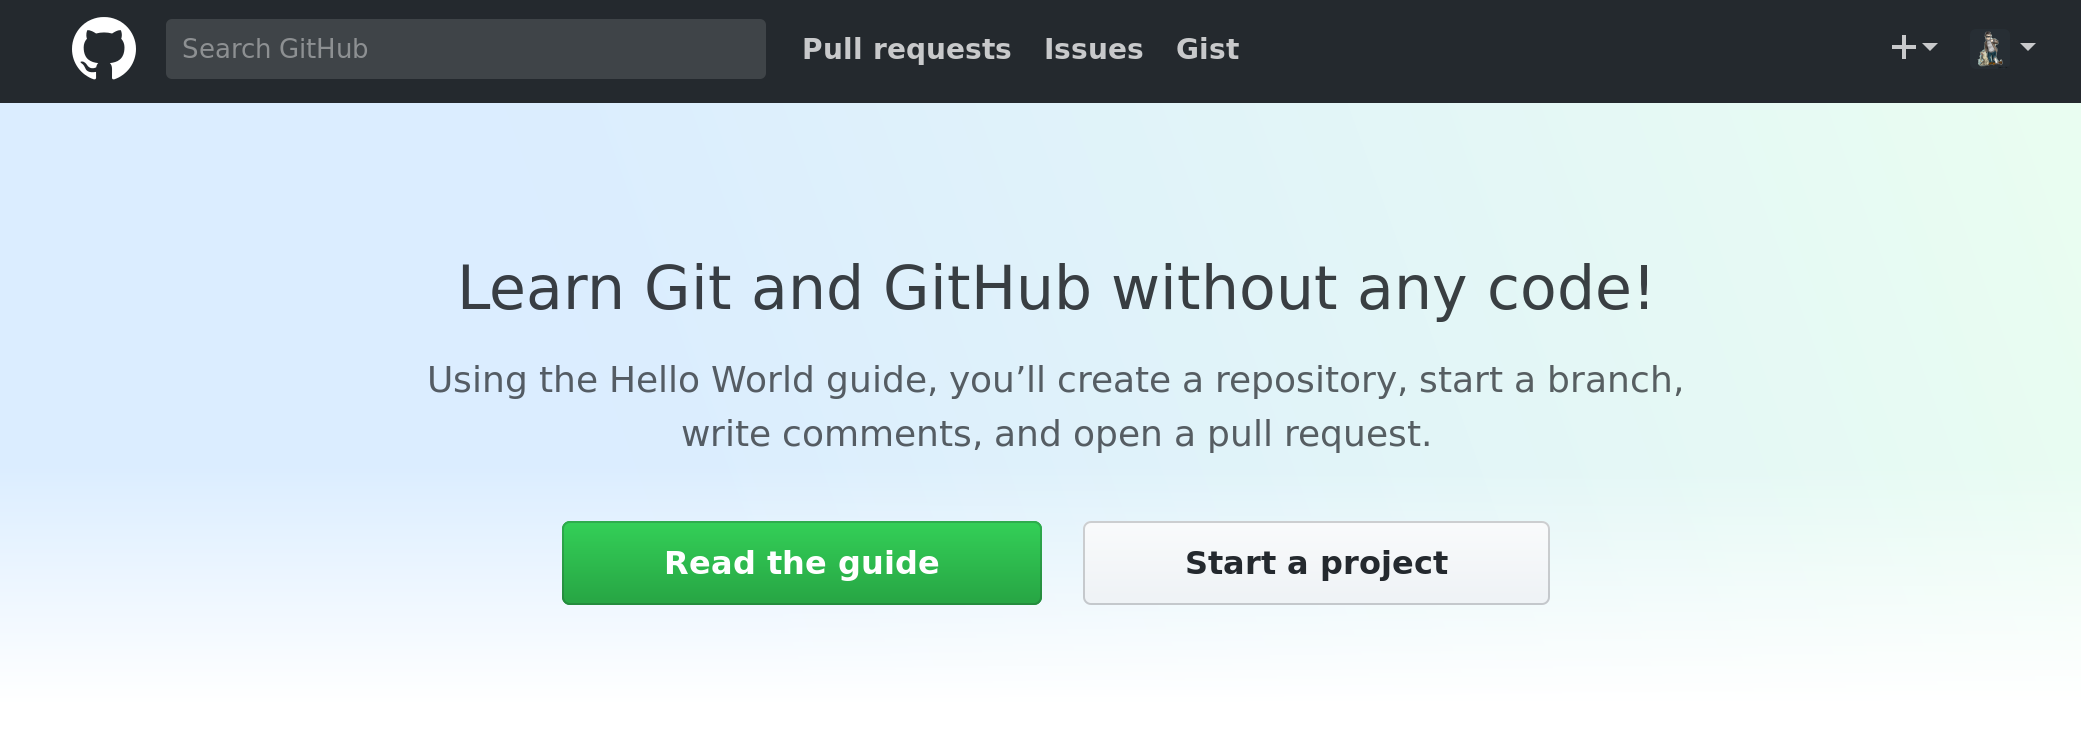
\includegraphics[width=0.75\textwidth]{fig/00start}
    % \caption{Sitio web de GitHub.}
    \label{fig:githw}
  \end{figure}
\end{frame}

\begin{frame}{GitHub: creando un repositorio}
  \begin{figure}[hp]
    \centering 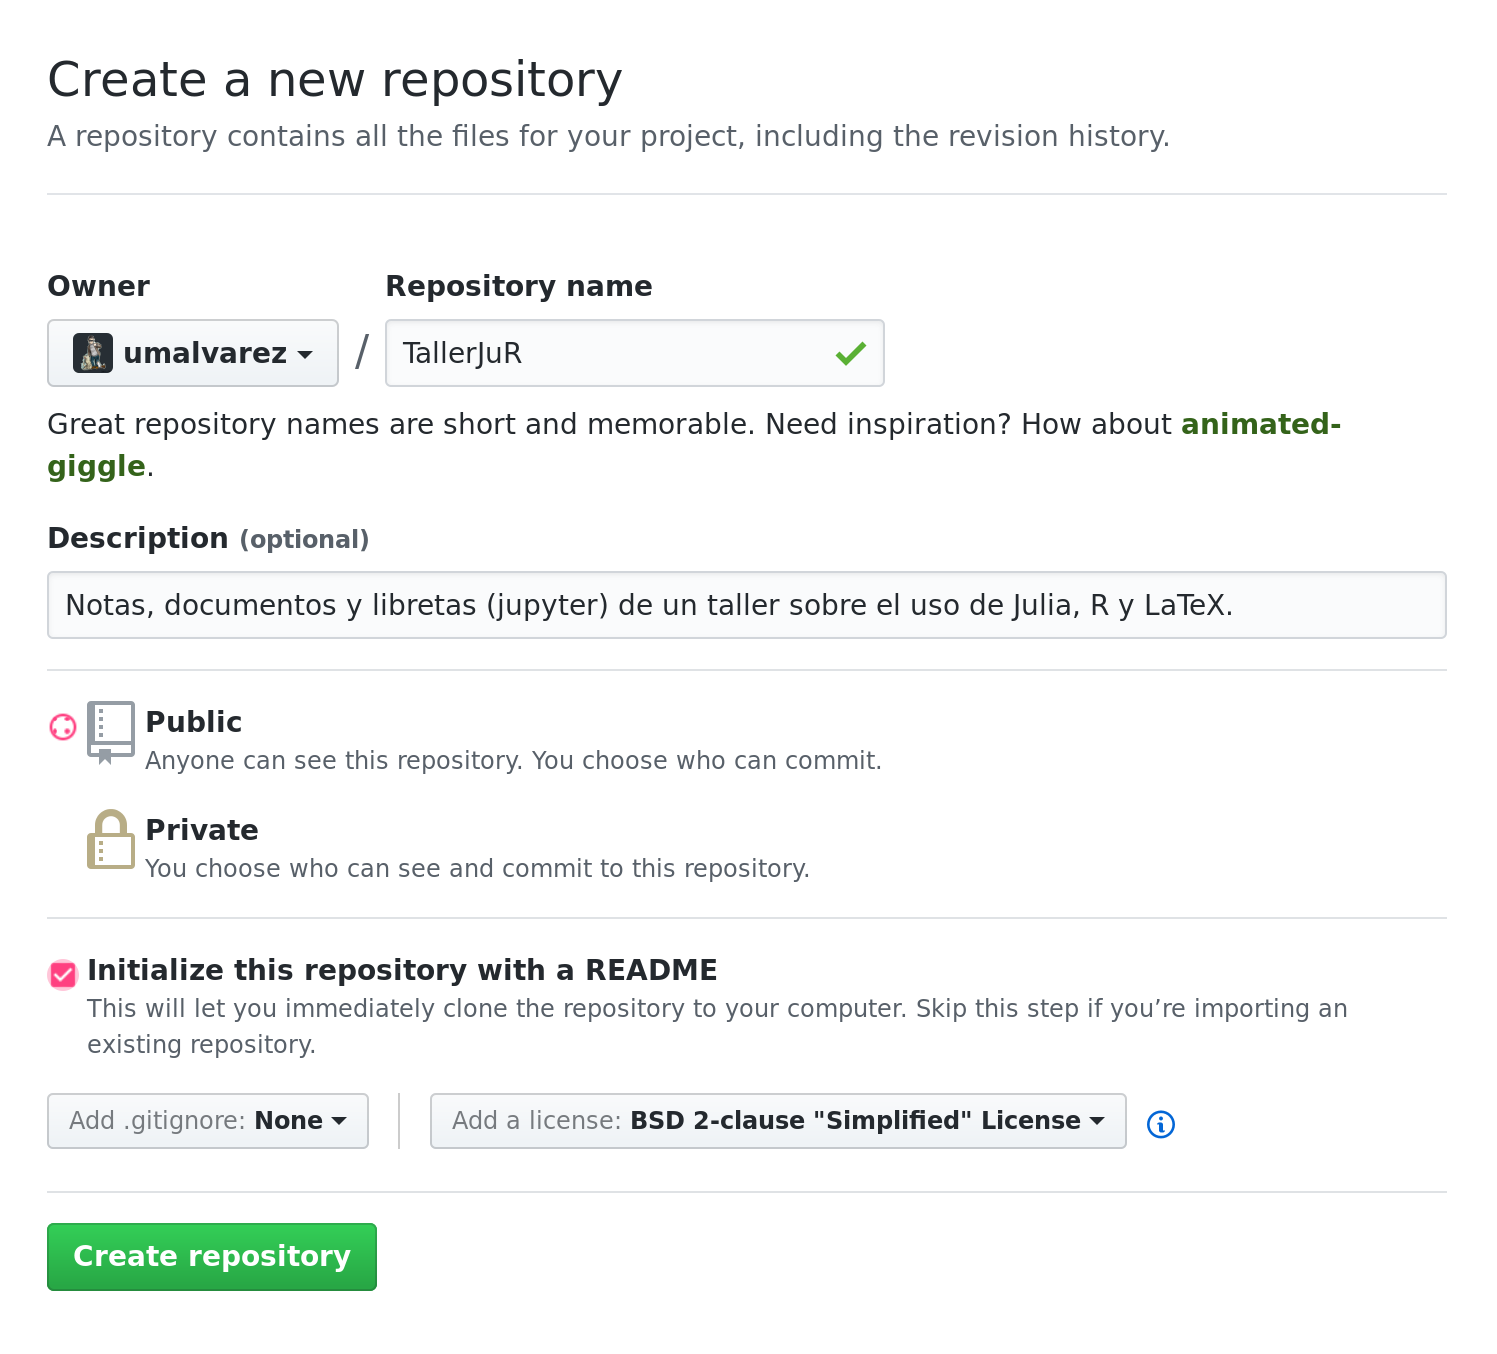
\includegraphics[width=0.75\textwidth]{fig/01newRepo}
    % \caption{Creando un nuevo repositorio.}
    \label{fig:githNr}
  \end{figure}
\end{frame}

\begin{frame}{GitHub: el primer repositorio}
  \begin{figure}[hp]
    \centering 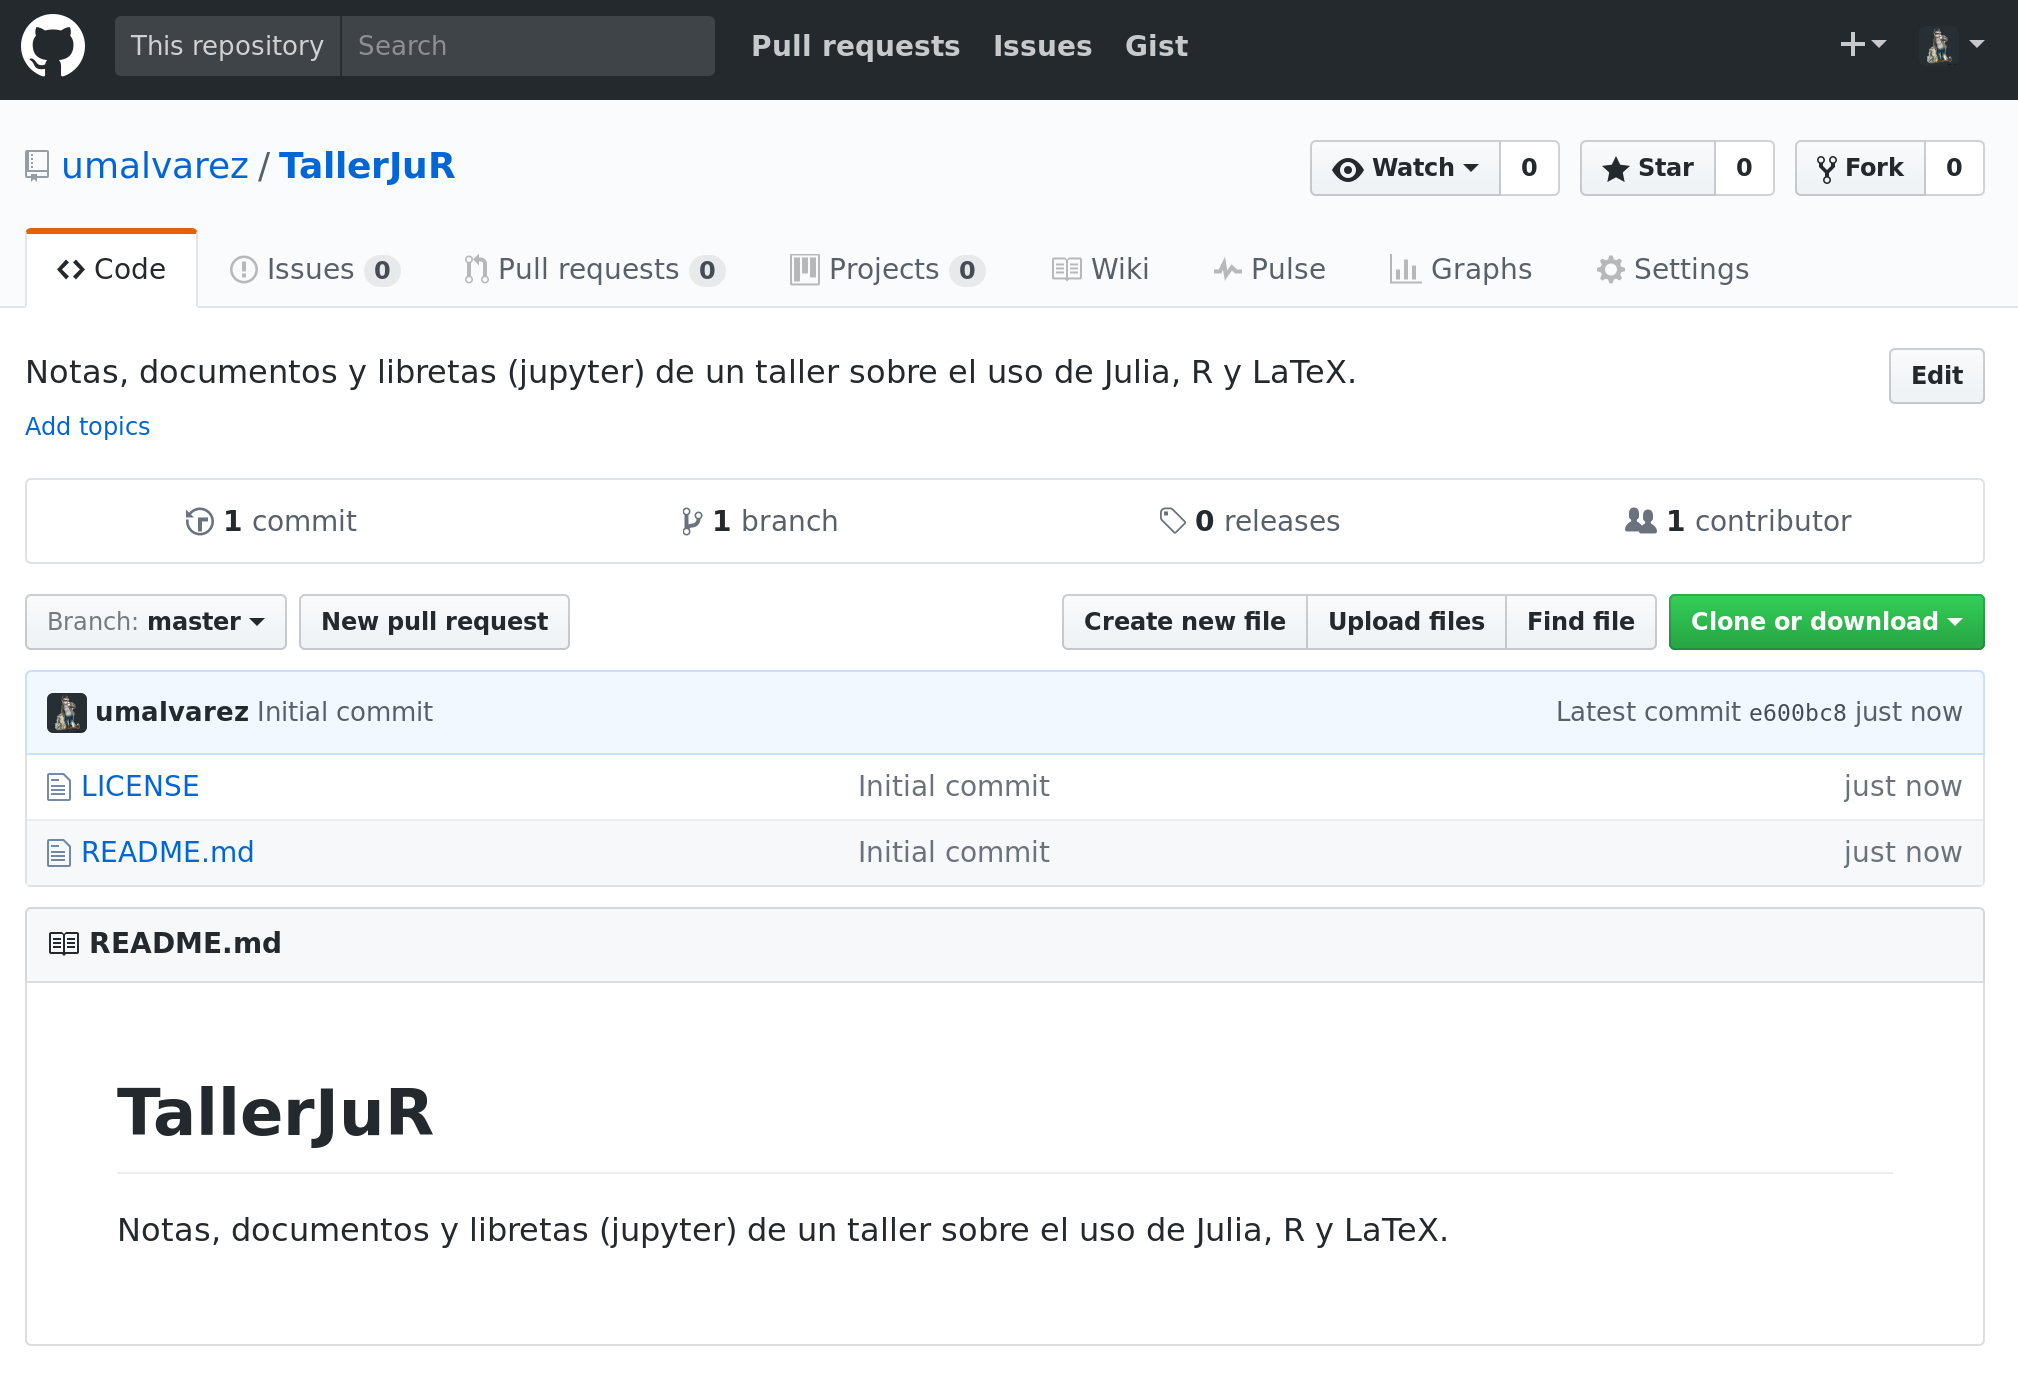
\includegraphics[width=0.75\textwidth]{fig/02The1stRepo}
    % \caption{Creando un nuevo repositorio.}
    \label{fig:git1st}
  \end{figure}
\end{frame}

\begin{frame}{GitHub: el primer env\'i{}o - I}
  \begin{figure}[hp]
    \centering 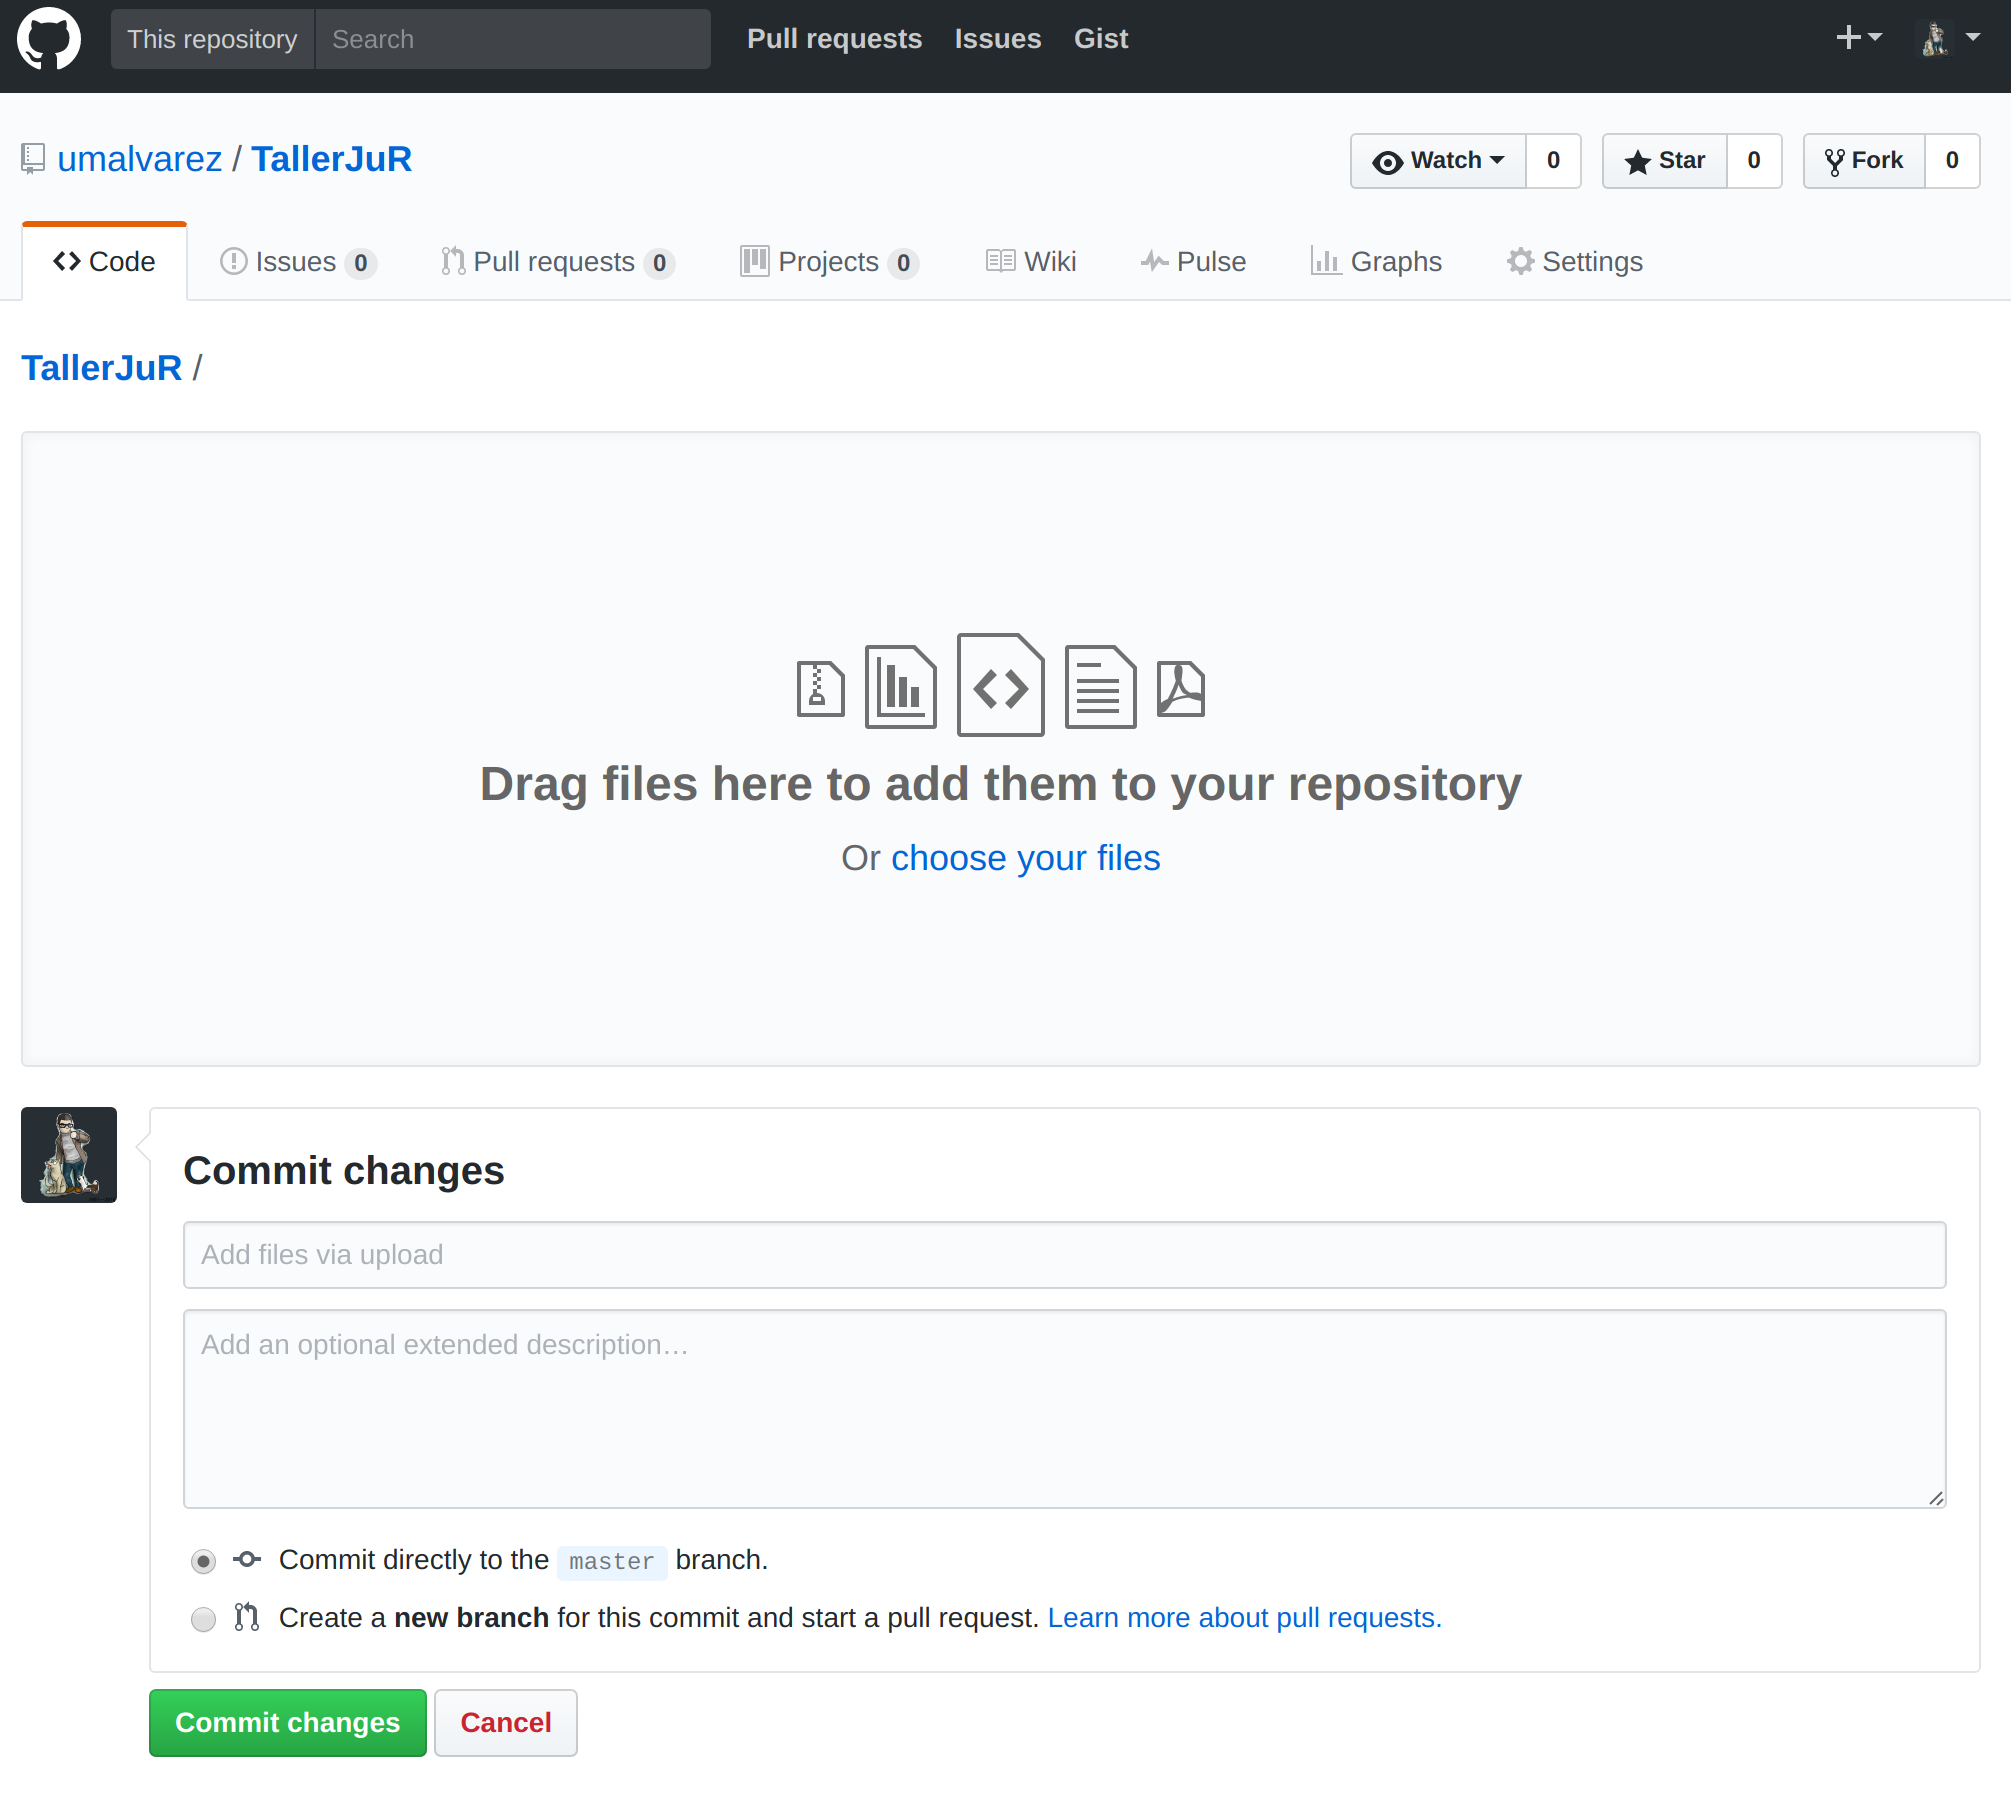
\includegraphics[width=0.75\textwidth]{fig/03The1stCommit}
    % \caption{Creando un nuevo repositorio.}
    \label{fig:git1stci}
  \end{figure}
\end{frame}

\begin{frame}{GitHub: el primer env\'i{}o - II}
  \begin{figure}[hp]
    \centering 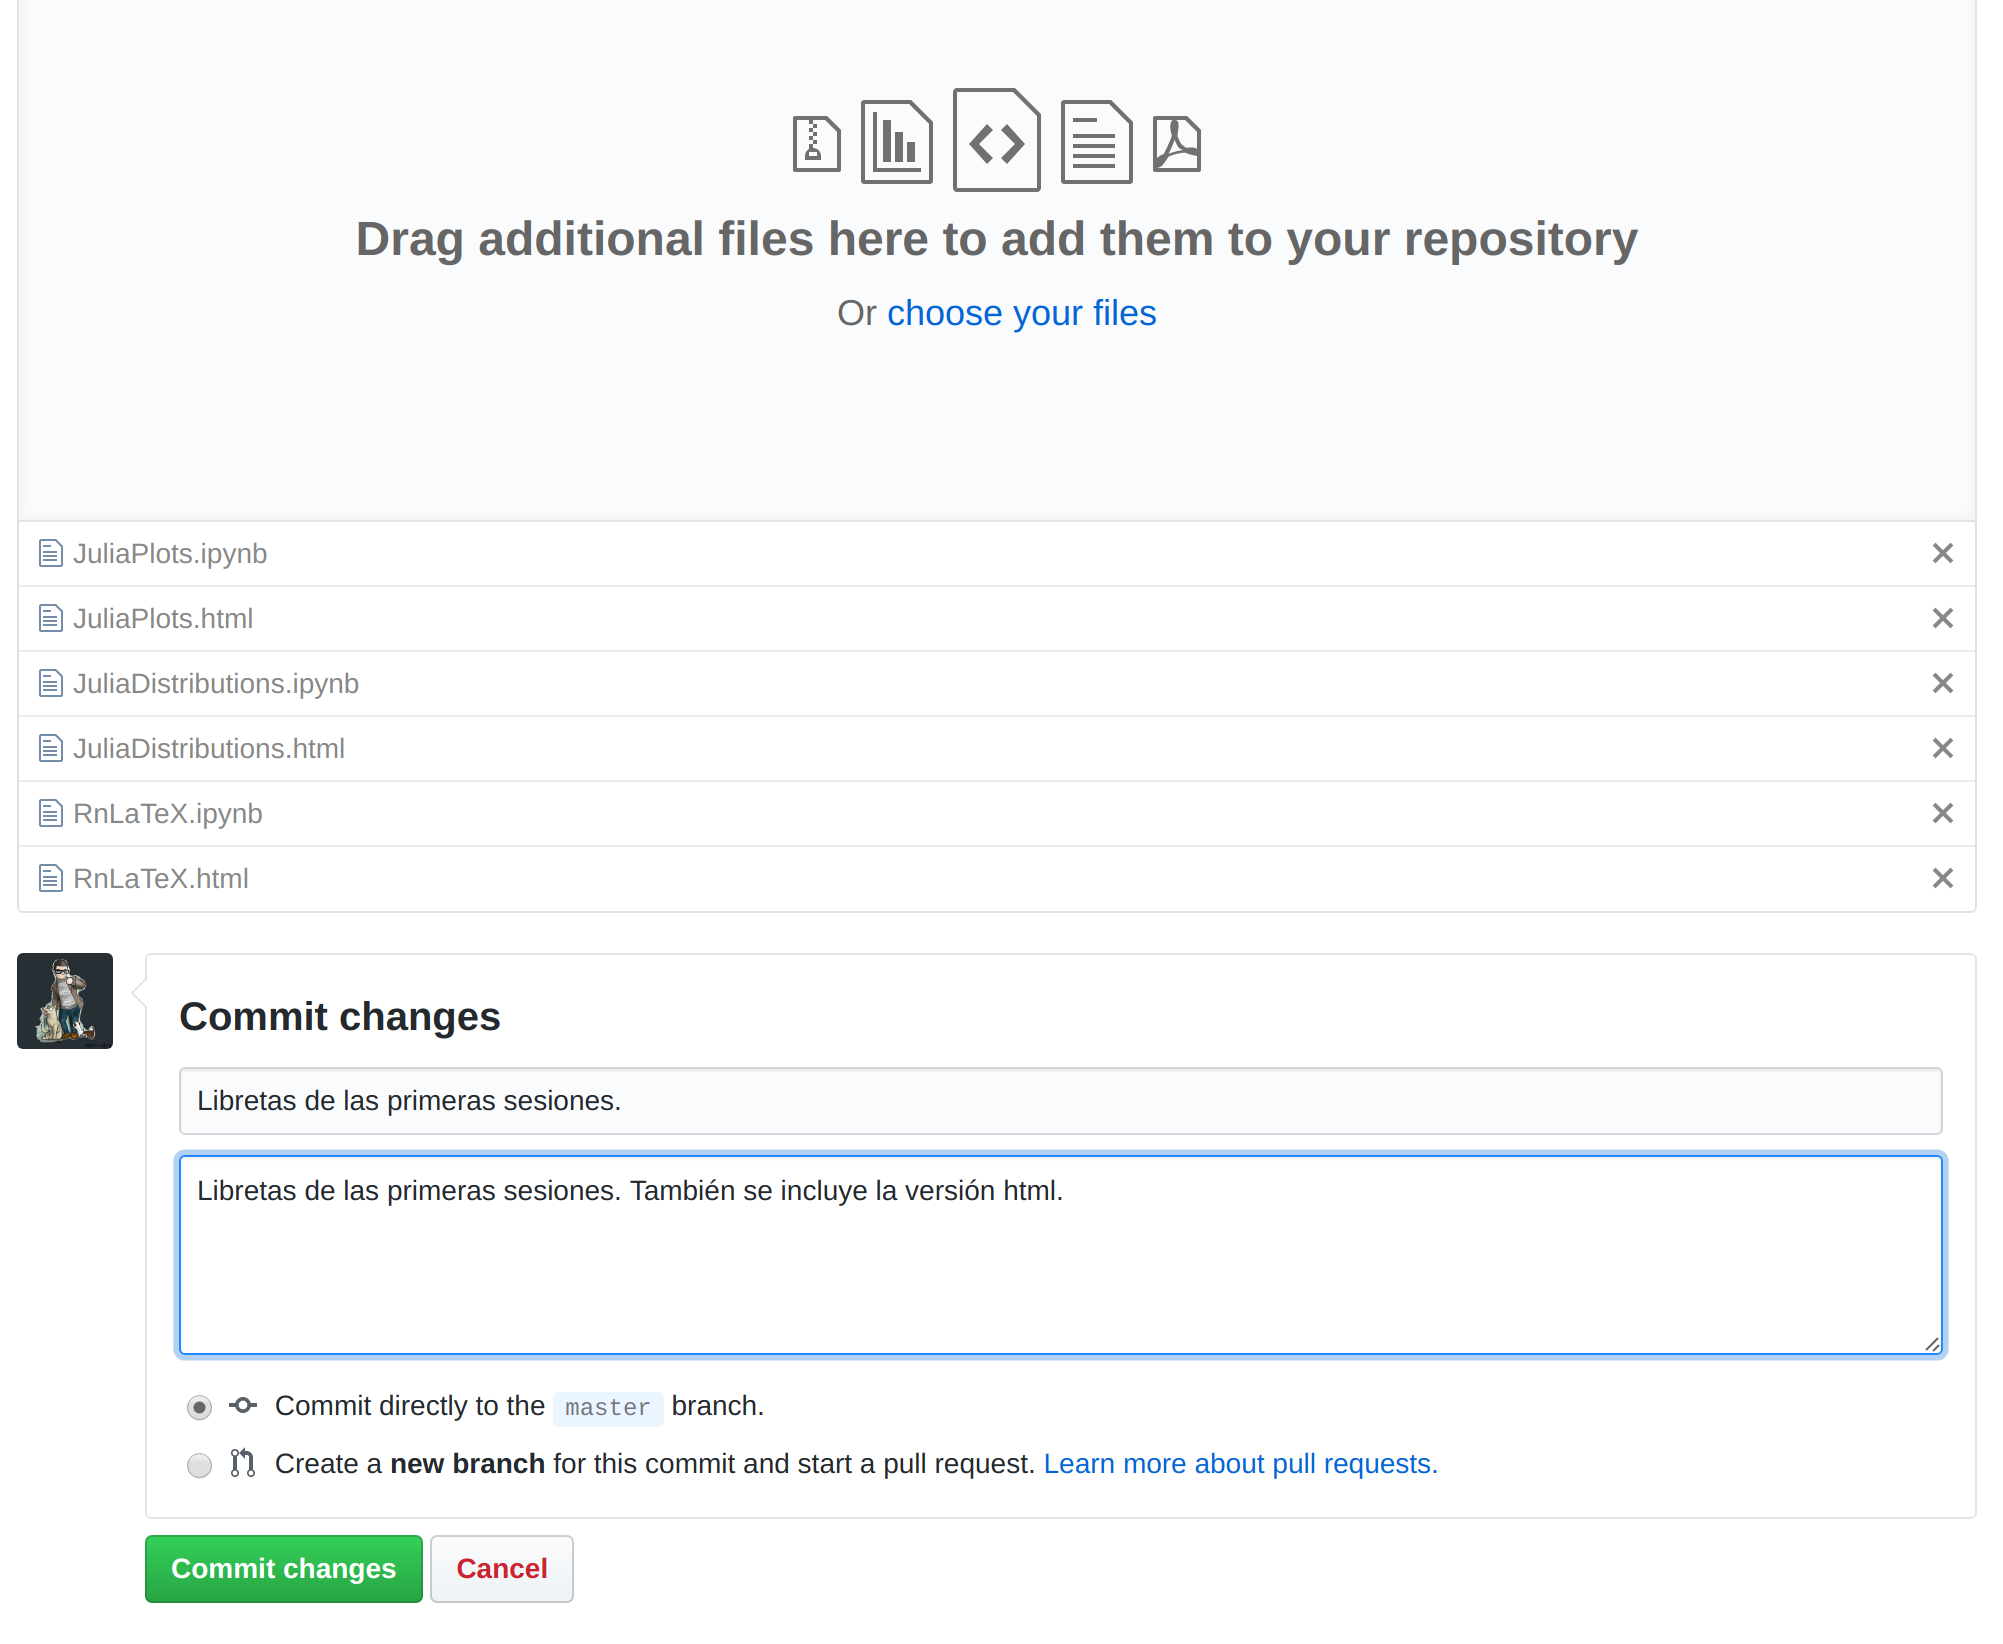
\includegraphics[width=0.75\textwidth]{fig/04The1stCommit}
    % \caption{Creando un nuevo repositorio.}
    \label{fig:git1stcii}
  \end{figure}
\end{frame}

\begin{frame}{GitHub: el primer env\'i{}o - III}
  \begin{figure}[hp]
    \centering 
\includegraphics[width=0.75\textwidth]{fig/05The1stCommit}
    % \caption{Creando un nuevo repositorio.}
    \label{fig:git1stciii}
  \end{figure}
\end{frame}

\begin{frame}{GitHub: el primer env\'i{}o - IV}
  \begin{figure}[hp]
    \centering 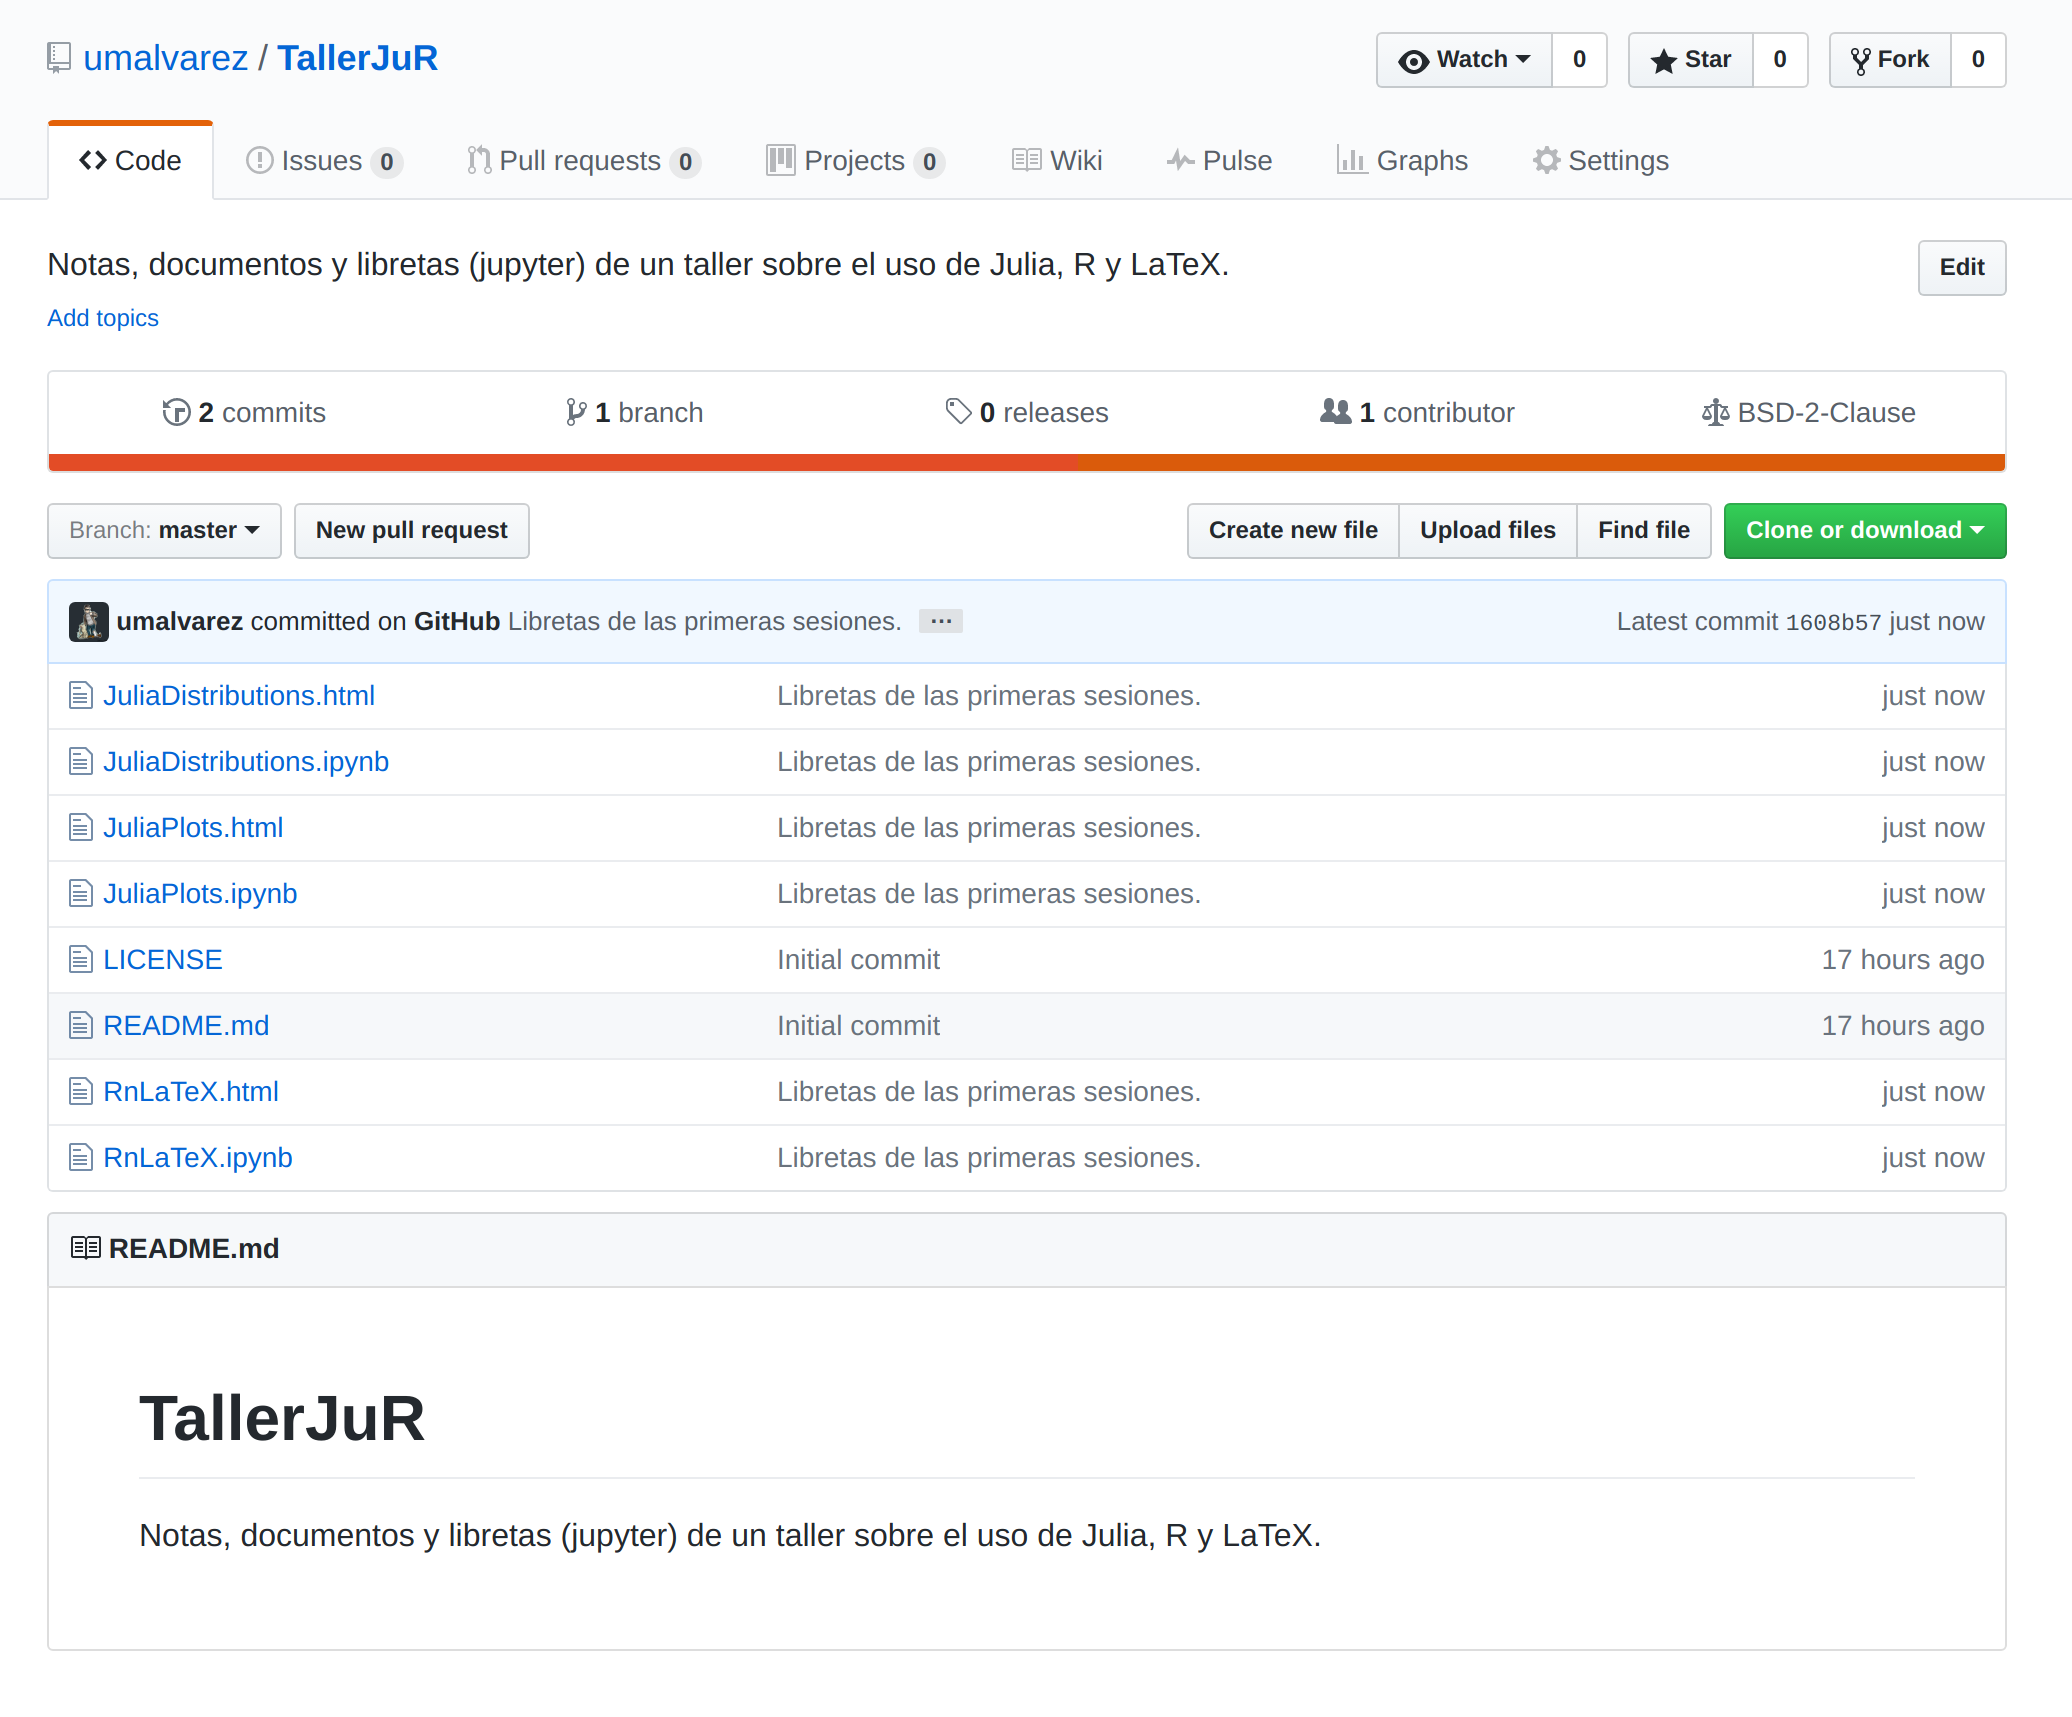
\includegraphics[width=0.75\textwidth]{fig/06The1stCommit}
    % \caption{Creando un nuevo repositorio.}
    \label{fig:git1stciv}
  \end{figure}
\end{frame}

\begin{frame}{GitHub: descargando o clonando el repositorio}
  \begin{figure}[hp]
    \centering 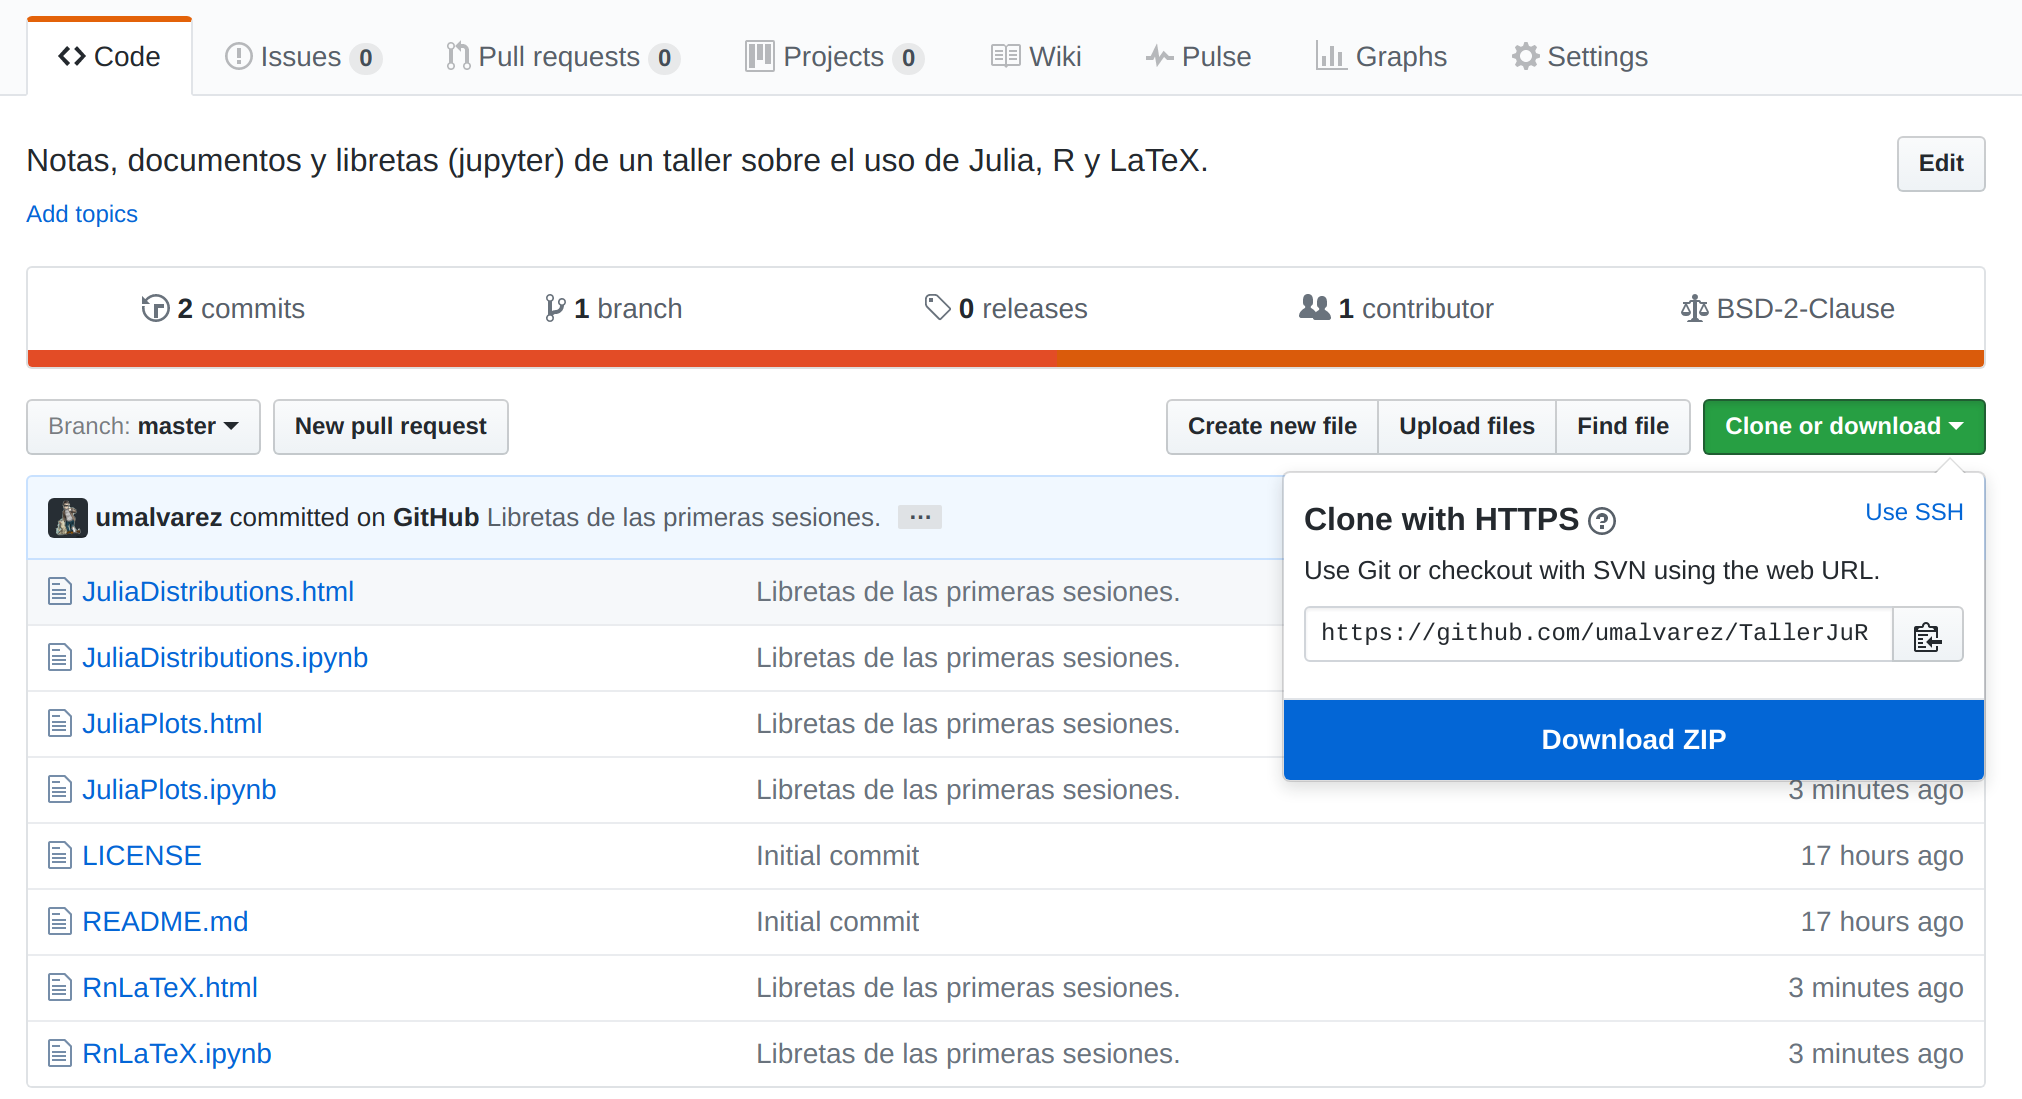
\includegraphics[width=0.75\textwidth]{fig/08Download}
    % \caption{Creando un nuevo repositorio.}
    \label{fig:gitclone}
  \end{figure}
\end{frame}


% % \section{Conclusiones}
% % \label{sec:conlusiones}


% \begin{frame}[standout]
%   Qué lenguaje usar
% \end{frame}

% \begin{frame}{Conclusiones}
%   \begin{itemize}
%   \item Lo que use mi gremio (\emph{siempre y cuando sea de código
%     abierto}).
%   \item El que se integre mejor a mi flujo de trabajo.
%   \item Perspectiva de desarrollo académico (\emph{no siempre el más
%     usado es el mejor}).
%   \end{itemize}
% \end{frame}


\end{document}
%%% Local Variables:
%%% mode: latex
%%% mode: flyspell
%%% TeX-engine: xetex
%%% End:
